\documentclass[UTF8,a4paper,12pt]{ctexbook} 

 \usepackage{graphicx}%学习插入图
 \usepackage{verbatim}%学习注释多行
 \usepackage{booktabs}%表格
 \usepackage{geometry}%图片
 \usepackage{amsmath}
 \usepackage{amssymb}
 \usepackage{listings}%代码
 \usepackage{xcolor}  %颜色
 \usepackage{enumitem}%列表格式
 \usepackage{tcolorbox}
 \usepackage{algorithm}  %format of the algorithm
 \usepackage{algorithmic}%format of the algorithm
 \usepackage{multirow}   %multirow for format of table
 \usepackage{tabularx} 	%表格排版格式控制
 \usepackage{array}	%表格排版格式控制
 \usepackage{hyperref} %超链接 \url{URL}
 % \setCJKmainfont{方正兰亭黑简体}  %中文字体设置
 % \setCJKsansfont{华康少女字体} %设置中文字体
 % \setCJKmonofont{华康少女字体} %设置中文字体

 \CTEXsetup[format+={\flushleft}]{section}
 \graphicspath{{figure/}}

 
 %%%% 下面的命令定义图表、算法、公式 %%%%
 \newcommand{\EQ}[1]{$\textbf{EQ:}#1\ $}
 \newcommand{\ALGORITHM}[1]{$\textbf{Algorithm:}#1\ $}
 \newcommand{\Figure}[1]{$\textbf{Figure }#1\ $}
 
 %%%% 下面命令改变图表下标题的前缀 %%%%% 如:图-1、Fig-1
 \renewcommand{\figurename}{Fig}
 
 \geometry{left=1.6cm,right=1.8cm,top=2cm,bottom=1.7cm} %设置文章宽度
 
 \pagestyle{plain} 		  %设置页面布局

 %代码效果定义
 \definecolor{mygreen}{rgb}{0,0.6,0}
 \definecolor{mygray}{rgb}{0.5,0.5,0.5}
 \definecolor{mymauve}{rgb}{0.58,0,0.82}
 \lstset{ %
 	backgroundcolor=\color{white},   % choose the background color
 	basicstyle=\footnotesize\ttfamily,      % size of fonts used for the code
 	%stringstyle=\color{codepurple},
 	%basicstyle=\footnotesize,
 	%breakatwhitespace=false,         
 	%breaklines=true,                 
 	%captionpos=b,                    
 	%keepspaces=true,                 
 	%numbers=left,                    
 	%numbersep=5pt,                  
 	%showspaces=false,                
 	%showstringspaces=false,
 	%showtabs=false,        
 	columns=fullflexible,
 	breaklines=true,                 % automatic line breaking only at whitespace
 	captionpos=b,                    % sets the caption-position to bottom
 	tabsize=4,
 	commentstyle=\color{mygreen},    % comment style
 	escapeinside={\%*}{*)},          % if you want to add LaTeX within your code
 	keywordstyle=\color{blue},       % keyword style
 	stringstyle=\color{mymauve}\ttfamily,     % string literal style
 	frame=L,
 	xleftmargin = .05\textwidth,
 	rulesepcolor=\color{red!20!green!20!blue!20},
 	% identifierstyle=\color{red},
 	language=php,
 }
 \author{\kaishu 郑华}
 \title{\heiti Redis笔记}
 
\begin{document}          %正文排版开始
 	\maketitle
  

\chapter{Redis 简介}
	\section{应用场景}
		\begin{itemize}
			\item 缓存
			\item 聊天室,秒杀,任务队列
			\item 需要精确设定过期时间的应用
			\item 应用排行榜.网站统计
			\item Pub/Sub构建实时消息系统:订阅、消息
			\item 数据存储(add,del,update,select)定期持久化到硬盘中
			\item 分布式集群架构中的session 分离
		\end{itemize}
		
	\section{安装与启动}
		\begin{lstlisting}
	// 安装
	$ wget http://download.redis.io/releases/redis-2.8.17.tar.gz
	$ tar xzf redis-2.8.17.tar.gz
	$ cd redis-2.8.17
	$ make	
	
	
	//启动redis服务.
	$ cd src
	$ ./redis-server
	
	//使用默认配置启动redis	服务
	./redis-server redis.conf
	
	//启动redis服务进程后,就可以使用测试客户端程序redis-cli和redis服务交互了	
	./redis-cli		
		\end{lstlisting}
	
	\section{配置}
		\begin{lstlisting}
	daemonize    如果需要在后台运行,把该项改为yes  
	pidfile      配置多个pid的地址 默认在/var/run/redis.pid
	bind 绑定ip,设置后只接受来自该ip的请求
	port 监听端口,默认为6379
	timeout      设置客户端连接时的超时时间,单位为秒
	loglevel     分为4级,debug、verbose、notice、warning
	logfile      配置log文件地址
	databases    设置数据库的个数,默认使用的数据库为0
	save         设置redis进行数据库镜像的频率
	rdbcompression    在进行镜像备份时,是否进行压缩
	Dbfilename        镜像备份文件的文件名
	Dir   数据库镜像备份的文件放置路径
	Slaveof     设置数据库为其他数据库的从数据库
	Masterauth 主数据库连接需要的密码验证
	Requirepass     设置登录时需要使用的密码
	Maxclients 限制同时连接的客户数量
	Maxmemory 设置redis能够使用的最大内存
	Appendonly 开启append only模式	
		\end{lstlisting}
\chapter{基本操作}	
	redis命令\textbf{不区分大小写},所以\verb|get var|和\verb|GET var|是等价的
	
	\section{选库}
		使用\textbf{Select} 命令用于\textit{切换到}\textbf{指定的数据库},数据库索引号 index 用数字值指定,以 0 作为起始索引值。
	
		flushdb \#清空数据库。
		
	\section{Key}
		\begin{table}[H]
			\centering
			\caption{常用命令}
			\begin{tabular}{p{5cm}<{\centering} | p{10cm}<{\centering}}
				\hline
					命令  &  含义 \\
				\hline
					\textbf{keys} [pattern] & 返回相应的的key \\
					\textbf{set} key value & 设定一个key-value \\
					\textbf{get} key &  获取一个key的值\\
					\textbf{dump} key & 序列化给定key,并返回序列化的值\\
					\textbf{randomkey} & 返回随机的key \\
					\textbf{exists} key & 判断key是否存在 \\
					\textbf{type} key & 返回key 存储的类型 \\
					\textbf{del} key &  删除key \\
					\textbf{expire} key seconds & 给key设置过期时间 \\
					\textbf{persist} key & 移除key 的过期时间,key将持久保存 \\
				\hline
			\end{tabular}
		\end{table}

	
	
\chapter{数据类型}	
	\section{string}
		\textbf{二进制安全的}。意思是redis的string可以包含任何数据。比如jpg图片或者序列化的对象 
		
		一个键最大能存储\verb|512MB|
		
		\begin{itemize}[itemindent = 1em] 
			\item \verb@set key value [ex 秒数]|[px 毫秒数]  [nx]|[xx]@	:设置键值
				\begin{itemize}
					\item \verb|nx |表示key 不存在时 执行操作
					\item \verb|xx |表示key 存在时 执行操作
					\item \verb|ex |表示设置 过期时间
					\item \verb|px |表示设置 持续时间,\verb|ex |与\verb|px |不能同时设置
				\end{itemize}
			\item \verb|mset key1 v1 key2 v2 ...| :一次性设置多个键值对(multi set) 			
			\item \verb|get key | 获取key 的值
			\item \verb|mget key1 key2 ...| :一次性获取多个键的值
			\item \verb|setrange key offset value |:把字符串的\verb|offset |偏移字节改为\verb|value|
				\begin{lstlisting}
	set greet hello
	get greet --> hello
	setrange greet 2 x
	get greet --> hexlo
	
	setrange greet 2 ??
	get greet --> he??o
	
	// 当偏移量大于字符长度时,多余部分将自动以0x00 填充
	setrange greet 6 !
	get greet --> he??o0x00!
				\end{lstlisting}
			\item \verb|append key value| :把value 追加到key 的原值上
			\item \verb|getrange key start stop| :获取字符串中 \verb|start, stop| 范围的值
				\begin{itemize}
					\item 左闭右闭区间,从0开始
					\item 负数 表示倒数第多少
				\end{itemize}
			
			\item \verb|getset key newValue| :获取并返回旧值,并设置新值
			\item \verb@incr|decr key@ :增1或减1,不存在的key 当成0再incr 返回。与之对应的有\verb|incrby key num|
			\item \verb|getbit key offset| :获取值的二进制的对应位上的值,从高位开始
			\item \verb|setbit key offset value| :设置对应2进制位上的值,offset 最长能达到\verb|2^32-1|位
			\item \verb|bitop op destKey key1 [key2 key3 ...]| :对[key1 key2..] 做op,并将结果保存到destKey 中,op 可以为一下几种\verb|AND OR NOT XOR|
		\end{itemize}
				
	\section{list -栈或队列}
		按照插入顺序排序。你可以添加一个元素到列表的头部(左边)或者尾部(右边)
		
		\begin{figure}[H]
			\centering
			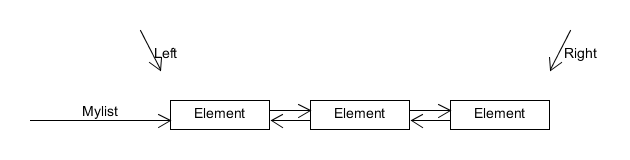
\includegraphics[scale=0.76]{list}
			\caption{链表结构}
		\end{figure}
		\begin{itemize}
			\item \textbf{lpush} \verb|mylist "hello" |:从头部插入字符串
			\item \textbf{rpush} \verb|mylist "world" |:从尾部插入字符串
			\item \textbf{lrange} \verb|mylist 0 -1 |:获取从0到倒数第一个,左右闭区间,如\verb|[1)hello 2)world]|
			\item \textbf{linsert} \verb|mylist before "hello" "start" |:在指定位置插入,与\verb|before| 对应的有 \verb|after|
			\item \textbf{lset} \verb|mylist 0 "Start" |:设置指定下标的值
			\item \textbf{lrem} \verb|mylist 1 "hello" |:删除(1个)值为hello 的元素,\verb|n = 0| 全部删除,\verb|n < 0|从尾部开始删除
			\item \textbf{lpop} \verb|mylist |:弹出开头的元素
			\item \textbf{rpop} \verb|mylist |:弹出结尾的元素
			\item \textbf{index} \verb|mylist 0 |:取出下标为0的元素值
			\item \textbf{llen} \verb|mylist |:返回表元素的个数
			\item \textbf{ltrim} \verb|mylist 0 2|:裁剪链表,保留从0号元素到2号元素之间的链表
		\end{itemize}
		
	\section{hash}
		\begin{figure}[H]
			\centering
			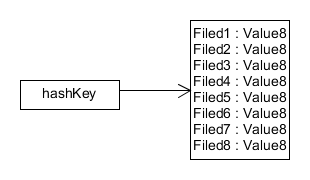
\includegraphics[scale=1]{hash}
			\caption{hash 结构}
		\end{figure}
		
		\begin{itemize}
			\item \verb|hset |user:001 name liweijie :哈希设置Key 为user:001,并增加域name,其键值为liweijie
			\item \verb|hsetnx |user:001 age 22 :检测键是否存在。若不存在创建
			\item \verb|hmset |user:002 name liweijie2 age 26 sex 1 :同时设置多个键的值
			\item \verb|hget |user:001 name :哈希获取Key user:001的name域的值。
			\item \verb|hmget |user:001 name age sex :获取多个指定的域键的值。
			\item \verb|hgetall |user:001 :获取所有当前key 域的值
			\item \verb|hincrby |user:001 age -8 :在指定域键上加上给定的值。
			\item \verb|hexists |user:001 sex :检测指定的域键是否存在。
			\item \verb|hlen |user:001 :返回指定哈希的键个数/字段个数
			\item \verb|hdel |user:001 sex :删除指定(user:001)哈希的指定字段或是键值。
			\item \verb|hkeys |user:003: 返回哈希里所有key。
		\end{itemize}		
		
	\section{set}
		Set 是 String 类型的无序集合。集合成员是唯一的,这就意味着集合中不能出现重复的数据。
		
		Redis 中集合是通过哈希表实现的,所以添加,删除,查找的复杂度都是 O(1)。
		
		\begin{itemize}
			\item \textbf{smembers} myset :查看myset集合中所有元素值。
			\item \textbf{sadd} myset "hello" :向mysets集合中添加一个值hello
			\item \textbf{srem} myset "hello" :删除myset集合中名称为hello的元素。
			\item \textbf{spop} myset  :随机弹出并返回mysets中的一个元素。
			\item \textbf{sdiff} myset2 myset3 :返回myset2中的与myset3的\textbf{差集}(以myset2为准)。
			\item \textbf{sdiffstore} myset4 myset2 myset3 :返回myset2中的与myset3的\textbf{差集},并存入myset4中去。
			\item \textbf{sinter} myset2 myset3 :返回myset2与myset3的交集。
			\item \textbf{sinterstore} myset5 myset2 myset3 :返回myset2与myset3的交集,并存入myset5中去。
			\item \textbf{sunion} myset2 myset3 :求并集
			\item \textbf{sunionstore} myset6 myset2 myset3 :求并集,并存入myset6中去。
			\item \textbf{smove} myset2 myset3 "three" :将myset2中的three移到myset3中去。
			\item \textbf{scard} myset2 :返回元素个数。
			\item \textbf{sismember} myset2 "one" :判断元素one是不是myset2集合的(相当于\verb|is_array()|)。
			\item \textbf{srandmember} myset2 :随机返回myset2集合中的一个元素,但不删除(相当于\verb|array_rand()|)。
		\end{itemize}
		
		\paragraph{集合的相关概念}
			\begin{itemize}
				\item 并集:以属于A或属于B的元素为元素的集合成为A与B的并(集) 
				\item 交集:以属于A且属于B的元素为元素的集合成为A与B的交(集) 
				\item 差:以属于A而不属于B的元素为元素的集合成为A与B的差(集)
			\end{itemize}
		
	\section{zset}
		有序集合和集合一样也是string类型元素的集合,\textbf{且不允许重复}的成员。
		
		\textit{不同的是每个元素都会关联一个double类型的分数}。redis正是通过分数来为集合中的成员进行从小到大的排序。
		
		有序集合的成员是唯一的,但分数(score)却可以重复。
		
		集合是通过\textbf{哈希表}实现的,所以添加,删除,查找的复杂度都是O(1)。
		\begin{itemize}
			\item \textbf{zadd} myZSet 1 zlh   :添加分数为1,值为zlh的zset集合,可多添加多组\verb|[socre2 value2]|
			\item \textbf{zcard} myZSet   :输出zset的成员个数
			\item \textbf{zrange} mZySet 0 -1 withscores :查看Zset指定范围的成员,withscores为输出结果带分数,0为开始,-1(倒数第一)为结束
			\item \textbf{zrank} mZySet Jim :获取zset成员的下标位置,如果值不存在返回null
			\item \textbf{zcount} mySet 1 3 :输出\verb| 分数>=1 and 分数 <=3 |的成员个数,因为分数是可以重复的,所以这个命令是有道理的
			\item \textbf{zrem} myZSet zlh :删除指定的一个成员或多个成员,\verb|[]|
			\item \textbf{zscore} myZset zlh :获取指定值的分数
			\item \textbf{zincrby} myZset 4 tom :给指定元素的分数进行增减操作,负值为减,正值为加
			\item \textbf{zrangebyscore} myZset :根据指定分数的范围获取值
				\begin{itemize}
					\item zrangebyscore myZset  1 5  :输出分数>=1 and <=5的成员值
					\item zrangebyscore myZset  (1 5  :输出分数>1 and <=5的成员值
					\item zrangebyscore myZset 2 5 limit 1 2  :检索分数为2到5之间的数据,然后从下标为1的数据开始往后输出2个数据,包含下标为1的数据
					\item zrangebyscore myZset -inf +inf limit 2 3 :+inf表示最后一个成员,-inf表示第一个成员,意思是:检索所有数据,然后从下标为2的数据开始再往后输出2个数据
				\end{itemize}
			\item \textbf{zrevrange},\textbf{zrevrangebyscore} :倒序,从高到底排序输出指定范围的数据
			\item \textbf{zremrangebyscore},\textbf{zremrangebyrank} :根据坐标,分数范围删除数据
			\item \textbf{zunionzstore} heZset 2 myZset youZset  :将myzset和youzset的\textbf{并集}添加到hezset中。
			\item \textbf{zinterstore} sheZset 2 myZset youZset  :将myzset和youZset 的交集添加到sheZset中。
		\end{itemize}

	\section{事务与锁}
		类似于mysql 的 start transaction, 可以保证原子性,可以使用rollback 取消操作。
		
		redis 使用 multi  命令实现
		
		使用 watch 锁,解决多用户竞争
		
		Redis 事务可以一次执行多个命令, 并且带有以下两个重要的保证:
			\begin{itemize}[itemindent = 2em]
				\item 批量操作在发送 EXEC 命令前被放入队列缓存。
				\item 收到 EXEC 命令后进入事务执行,事务中任意命令执行失败,其余的命令依然被执行。
				\item 在事务执行过程,其他客户端提交的命令请求不会插入到事务执行命令序列中。
			\end{itemize}
		
		一个事务从开始到执行会经历以下三个阶段:
			\begin{enumerate}[itemindent = 2em]
				\item 开始事务。
				\item 命令入队。\textit{如果中间存在错误,事务执行取消}
				\item 执行事务。
			\end{enumerate}
		
		\begin{table}[H]
			\centering
			\caption{事务与锁 操作说明}
			\begin{tabular}{p{5cm}<{\centering} | p{10cm}<{\centering}}
				\toprule
					命令 &  含义 \\
				\midrule
				\textbf{MULTI} 	 &  标记一个事务块的开始。	\\
				\textbf{EXEC} 	 & 	执行所有事务块内的命令。	\\
				\textbf{DISCARD} 	 &	取消事务,放弃执行事务块内的所有命令。	\\
				\textbf{UNWATCH} 	 &	取消 WATCH 命令对所有 key 的监视。	\\
				\textbf{WATCH} key [key ...] 	 &	监视一个(或多个) key ,如果在事务执行之前这个(或这些) key 被其他命令所改动,那么事务将被打断。	\\
				\bottomrule
			\end{tabular}
		\end{table}

\chapter{订阅与发布}
	Observer 观察者模式
	
	\section{publish 主题  消息} 声明、发布 主题,并提供消息。
	
	\section{subscribe 主题} 收听、监听、订阅 某主题

	\section{psubscribe 主题模式} 收听某种正则规则的主题
	
\chapter{持久化}	
	\section{rdb 持久化}
		\begin{figure}[H]
			\centering
			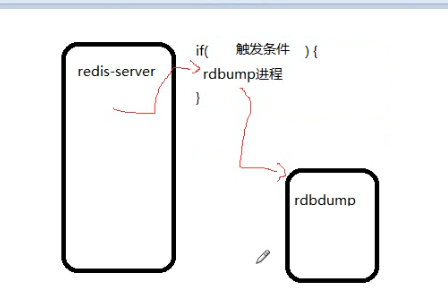
\includegraphics[scale=1]{rdb}
			\caption{镜像备份原理}
		\end{figure}
			
		\paragraph{SAVE|BGSAVE}
			用于创建当前数据库的备份。
			
			\subparagraph{相关参数}
				\begin{itemize}[itemindent = 1em]
					\item \verb|save 900 1| :刷新快照到硬盘中,必须满足900秒后至少有一个关键字发生变化
					\item \verb|save 300 10| :必须是300秒以后至少10个关键字发生变化
					\item \verb|save 60 10000|:必须是60秒以后至少10000个关键字发生变化
					\item \verb|stop-writes-on-bgsave-error yes|:后台存储进程出错时,前端缓存不允许写操作,既改变关键字
					\item \verb|rdbcompression yes|:使用LZF压缩rdb 文件
					\item \verb|dbfilename dump.rdb|:设置rdb文件名
					\item \verb|dir ./|:设置备份保存路径
				\end{itemize}
				
		\paragraph{恢复数据}
			如果需要恢复数据,只需将备份文件 (dump.rdb) \textbf{移动到} \verb|redis| \textbf{安装目录}并启动服务即可。
			
			获取 redis 目录可以使用 CONFIG 命令:\verb|CONFIG GET dir|
	
		\paragraph{特点}
			恢复数据快,镜像恢复,但是可能存在数据丢失(当断电时没有触发备份条件)。
		
	\section{aof 持久化}
		\begin{figure}[H]
			\centering
			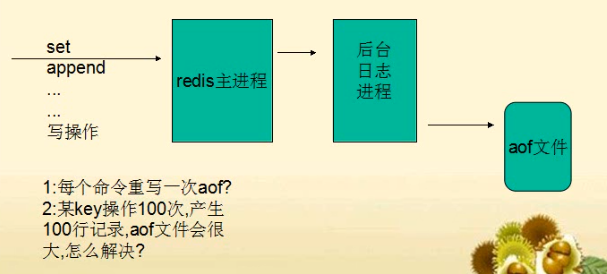
\includegraphics[scale=0.9]{rof}
			\caption{aof 备份原理}
		\end{figure}

		\paragraph{Aof 配置}
			\begin{itemize}
				\item \verb|appendonly on| :是否打开aof 日志功能
				\item \verb|appendfsync always |:每1个命令,都立即同步到aof,安全,速度慢
				\item \verb|appendfsync every sec |:折衷方案,每秒写一次
				\item \verb|appendfsync no |:写入工作交给操作系统,由操作系统判断缓冲区大小统一写入到aof,同步频率低,速度快
				\item \verb|no-appendfsync-on-rewrite  yes |: 正在导出rdb 快照的过程中,要不要停止同步aof
				\item \verb|auto-aof-rewrite-percentage 100 |:aof文件大小比上次重写时的大小,增长率100\% 时,重写
				\item \verb|auto-aof-rewrite-min-size-64mb |:aof文件至少超过64MB时重写
			\end{itemize}
		
			\subparagraph{Aof 重写 BGREWRITE}
				aof 重写是指把内存中的数据,逆化成命令,简化命令个数,写入到aof 日志里,以解决aof 日志过大的问题。	
			
			\subparagraph{当rdb 和 aof同时存在时}
				\begin{itemize}[itemindent = 1em]
					\item 当有aof文件时, 使用aof恢复数据,否则使用rdb
					\item 在恢复速度上,rdb因为是直接的内存映射,而aof 是逐条运行命令,因此在速度上来说rdb 比aof 快很多。
				\end{itemize}

\chapter{分布式}	
	\section{主从复制}
		\begin{itemize}
			\item 主从备份,防止主机宕机
			\item 读写分离,分担master 的任务
			\item 任务分离,从服分别担任不同的工作(备份、计算)
		\end{itemize}
		
		\begin{figure}[H]
			\centering
			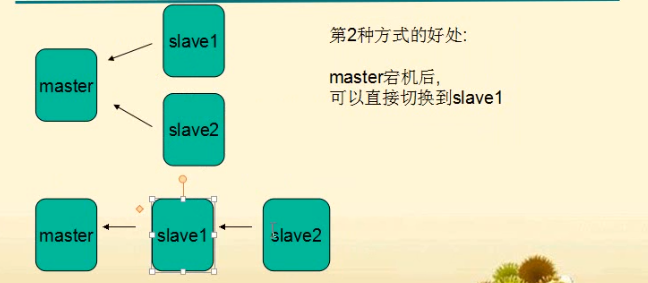
\includegraphics[scale=.7]{slave}
			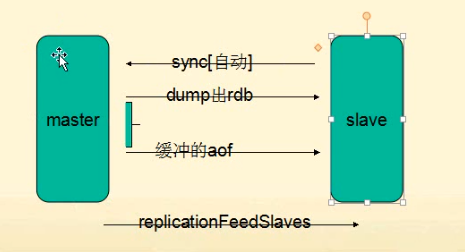
\includegraphics[scale=1]{slaveCom}
			\caption{主从2种结构、通信方式}
		\end{figure}
		

		
		
	\section{分布式集群}
		 \begin{figure}[H]
				\centering
				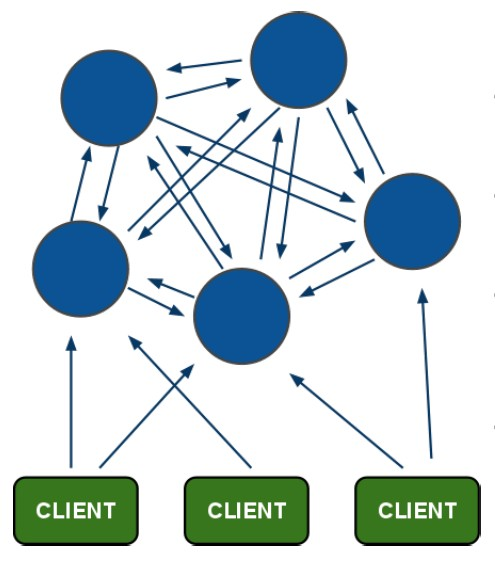
\includegraphics[scale=0.5]{cluster}
				\caption{Redis 集群示意}
		 \end{figure}
		 
		在这个图中,每一个蓝色的圈都代表着一个redis的服务器节点。它们任何两个节点之间都是相互连通的。客户端可以与任何一个节点相连接,然后就可以访问集群中的任何一个节点。对其进行存取和其他操作。
		
		还有就是因为如果集群的话,是有好多个redis一起工作的,那么,就需要这个集群不是那么容易挂掉,所以呢,理论上就应该给集群中的每个节点至少一个备用的redis服务。这个备用的redis称为从节点(slave)。那么这个集群是如何判断是否有某个节点挂掉了呢?
		
		首先要说的是,每一个节点都存有这个集群所有主节点以及从节点的信息。
			
		它们之间通过互相的ping-pong判断是否节点可以连接上。如果有一半以上的节点去ping一个节点的时候没有回应,集群就认为这个节点宕机了,然后去连接它的备用节点。如果某个节点和所有从节点全部挂掉,我们集群就进入faill状态。还有就是如果有一半以上的主节点宕机,那么我们集群同样进入发力了状态。这就是我们的redis的投票机制,具体原理如下图所示:
			\begin{figure}[H]
				\centering
				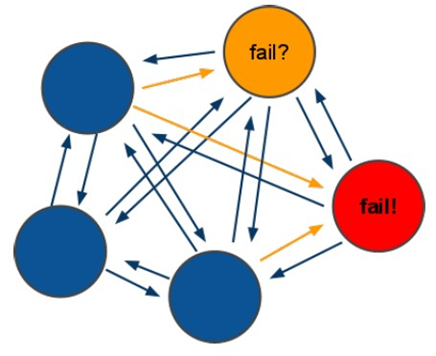
\includegraphics[scale=0.5]{failed}
				\caption{宕机演示}
			\end{figure} 	
		
		\begin{enumerate}
			\item 投票过程是集群中所有\verb|master|参与,如果\textbf{半数以上master节点}与\verb|master节点|通信超时(cluster-node-timeout),认为当前master节点\textbf{挂掉}.
			\item 什么时候整个集群不可用(\verb|cluster_state:fail|)?
				\begin{itemize}
					\item 如果集群任意master挂掉,且当前master没有slave.\textbf{集群进入fail状态},也可以理解成集群的slot映射[0-16383]不完整时进入fail状态. 
					\item 如果集群超过半数以上master挂掉,无论是否有slave,\textbf{集群进入fail状态}.
				\end{itemize}
		\end{enumerate}
			
		\subsection{参考}
			\begin{itemize}
				\item \url{https://www.cnblogs.com/yuanermen/p/5717885.html}
				\item \url{https://www.cnblogs.com/cjsblog/p/9048545.html}
				\item Redis Cluster 原理:\url{https://www.cnblogs.com/liyasong/p/redis_jiqun.html?utm_source=itdadao&utm_medium=referral}
				\item Redis Cluster:\url{http://www.cnblogs.com/foxmailed/p/3630875.html}
				\item 集群实践方案:\url{http://itindex.net/detail/51037-redis-%E5%AE%9E%E8%B7%B5-%E9%9B%86%E7%BE%A4}
			\end{itemize}
		
		
	\section{Redis分区}
		Redis Cluster 是\textbf{Redis的集群实现},内置数据\textbf{自动分片}机制,集群内部\textbf{将所有的key映射到16384个Slot中},集群中的\textbf{每个Redis Instance负责其中的一部分的Slot的读写}。集群客户端连接集群中任一Redis Instance即可发送命令,\textit{当Redis Instance收到自己不负责的Slot的请求时,会将负责请求Key所在Slot的Redis Instance地址返回给客户端,客户端收到后自动将原请求重新发往这个地址,对外部透明}。\textbf{一个Key到底属于哪个Slot由crc16(key) \% 16384 决定}。
				
		 \textbf{关于负载均衡},\textbf{集群的Redis Instance之间可以迁移数据},\textbf{以Slot为单位},但不是自动的,\textbf{需要外部命令触发}。
			
		 \textbf{关于集群成员管理},集群的节点(Redis Instance)和节点之间两两定期交换集群内节点信息并且更新,从发送节点的角度看,这些信息包括:集群内有哪些节点,IP和PORT是什么,节点名字是什么,节点的状态(比如OK,PFAIL,FAIL,后面详述)是什么,包括节点角色(master 或者 slave)等。
			
		 \textbf{关于可用性},\textbf{集群由N组主从Redis Instance组成}。主可以没有从,但是没有从 意味着主宕机后主负责的Slot读写服务不可用。\textbf{一个主可以有多个从,主宕机时,某个从会被提升为主,具体哪个从被提升为主,协议类似于Raft},参见这里。\textbf{如何检测主宕机?Redis Cluster采用quorum+心跳的机制}。从节点的角度看,节点会定期给其他所有的节点发送Ping,cluster-node-timeout(可配置,秒级)时间内没有收到对方的回复,则单方面认为对端节点宕机,将该节点标为PFAIL状态。通过节点之间交换信息收集到quorum个节点都认为这个节点为PFAIL,则将该节点标记为FAIL,并且将其发送给其他所有节点,其他所有节点收到后立即认为该节点宕机。从这里可以看出,主宕机后,至少cluster-node-timeout时间内该主所负责的Slot的读写服务不可用。
				 
		Redis集群的目的是实现数据的横向伸缩,把一块数据分片保存到多个机器,可以横向扩展数据库大小,扩展带宽,计算能力等。 
		
		分区是分割数据到多个Redis实例的处理过程,因此每个实例只保存key的一个子集。

		\paragraph{分区的优势}
			\begin{itemize}
				\item 通过利用多台计算机内存的和值,允许我们构造更大的数据库。
				\item 通过多核和多台计算机,允许我们扩展计算能力;通过多台计算机和网络适配器,允许我们扩展网络带宽。
			\end{itemize}
		
		redis集群大多数支持在\textbf{运行时}\textit{增加、删除节点}的透明数据平衡的能力,但是类似于客户端分区、代理等其他系统则不支持这项特性。然而,一种叫做\verb|presharding|的技术对此是有帮助的。
		
		\paragraph{分区类型}
			\begin{itemize}
				\item 范围分区:0-1000,1001-2000,..
				\item 哈希分区:
			\end{itemize}
			
\chapter{应用}	
	\section{位图法统计活跃用户}
		\begin{itemize}
			\item 1亿个用户
			\item 如何记录用户的登录信息
			\item 如何查询活跃用户,一周连续登录
		\end{itemize}
	
		从信息的角度看,一个用户的登录只需要 一个位 就可以表示。 0-1
		
		在数据库中,数据一般都有编号
		
		简化如:
			\begin{lstlisting}
	7个用户
	
	周一 01011100
	周二 01010010
	周三 01111000
	
	setbit  mon   100000000  0  // 初始化为0
	setbit  mon   3     1       // 第3号用户登录,标记为1
	setbit  mon   9     1
	
	
	setbit  tuseday 10000000 0
	set bit tuesday 4  1
	

	bitop and mon tuseday ...
	
			\end{lstlisting}
	\section{频道发布与订阅}
	
	\section{微博之用户注册与微博发布}
	
	\section{微博之粉丝关系与推送微博}
	
	\section{哈希数据存储微博}



\chapter{PHP 与 Redis}
	\section{关联}
		\begin{lstlisting}
	$redis = new redis();  
	$result = $redis->connect('127.0.0.1', 6379);  
	var_dump($result); //结果:bool(true)  
	
	$result = $redis->set('test',"11111111111");  
	var_dump($result);    //结果:bool(true)  
	
	$result = $redis->get('test');  
	var_dump($result);   //结果:string(11) "11111111111"  
	
	$redis->delete('test');  
	var_dump($redis->get('test'));  //结果:bool(false)  
		\end{lstlisting}		    
\end{document} 
 		    